\chapter{Real-case simulation}
\label{chap:real_case}

\section{Introduction}
In this chapter, we examine the behaviour of Pangolin forced with realistic
winds from meteorological analyses and with the introduction of a linearized
chemistry scheme for ozone. Since our goal is to obtain in the long run a complete
CTM based on Pangolin environment, this study is a natural extension of the
previous simulations described in Chapter~\ref{chap:testing}, in which  the  2D
advection was only tested with idealised tracer evolutions. 

To validate the simulations, the results of Pangolin are compared to those of the
MOCAGE CTM described in Section~\ref{subsec:mocage}. MOCAGE includes a full 3D
transport scheme so, since the advection scheme of Pangolin is only 2D, we
focus on the advection on an isentropic surface located in the mid-stratosphere.
Diabatic processes in the mid-stratosphere are dominated by radiation, which
induces rather small net heating rates at those altitudes. It is therefore relevant
to consider that on time scales of several days the air motions are mostly
adiabatic.
Here, we examine a simple chemistry scheme for ozone, where the ozone
concentration does not depends on other species. The configuration used for the
simulations is highlighted in Section~\ref{sec:config}. Results of Pangolin results are
shown in Section~\ref{sec:results_final}, along with a comparison to the results
of MOCAGE\@.

\section{Model set up}
\label{sec:config}
We have chosen stratospheric ozone as it is a good candidate for
studying the advection and its interference with chemistry. Simulations in the
stratosphere are also relevant for climatic applications as ozone is a key
component of the temperature balance at those altitudes. Stratospheric ozone
distribution has also been extensively monitored for several decades using remote
sensing instruments onboard satellites, providing useful datasets for model
validation.  In the stratosphere ozone is produced by photodissociation of
molecular oxygen. This production is balanced by destruction by catalytic cycles
involving NOx and HOx radicals.  Ozone lifetime is in the range of several days
at the equator in the mid-stratosphere, a time scale comparable to the advection
around the polar vortices. We have therefore chosen to focus our analysis on an
altitude close to 30 km for the month of september 2008, a period for which we
had previously performed simulations with the MOCAGE model.
 
\subsection{Meteorological data}
A chemistry-transport model can be used in either an \textit{online} or
\textit{offline} setup. In an online setup, the chemistry is directly integrated
into \glspl{GCM}. In this case, accessing the
meteorological data (pressure, temperature) from the dynamics is not an issue.
However, in Pangolin, we are in an offline setup: the \gls{CTM} is external to
fhe \gls{GCM} and the two must be coupled. The most common strategy is to use
desynchronised coupling. Noting $\Delta t$ the timestep of the coupling, an
iteration in the coupling would be:
\begin{enumerate}
\item chemical species are passed from the CTM to the GCM,
\item the GCM is integrated during $\Delta t$,
\item meteorological data are passed back to the CTM,
\item the CTM is integrated during $\Delta t$.
\end{enumerate}
$\Delta t$ is usually 3 to 6 hours. A shorter time-step would be expensive,
while a longer time-step would create some bias between the data of the CTM and
GCM, mostly due to the parametrization of unresolved processes (turbulence,
convection). 

In our study we use the data from the ECMWF \textit{re-analyses} to force both
MOCAGE and Pangolin. To obtain these re-analyses, observational data is
assimilated a first time, then fed to the model. The output of the model is then
assimilated again to match observational data at the next date.  Here, Pangolin
and MOCAGE are integrated using assimilated winds and temperature every three
hours. The initial ozone distribution on the 1st of September comes from an
analysis using the MOCAGE-VALENTINA suite (\cite{Emili2014}).

As the advection and chemistry time-steps are smaller than 3
hours, we added a temporal interpolation for the necessary data (temperature and
winds) at the required steps. Input winds at $t$ and $t+\Delta t$ are already corrected from
the preprocessing step (Section~\ref{subsec:spatial_interp}) and the
interpolation is linear so the interpolated winds remain non divergent.

\subsection{Treatment of the vertical outputs of MOCAGE  and Pangolin}
\label{subsec:vertical}
In 3D models, several sets of vertical coordinates can be used. The first is to
use simply pressure coordinates, which has the disadvantage of not taking the
landscape (mountains for example) into account. A solution to that would be to
use the latitude over the landscape but we would lose the pressure
information. Another set of coordinates uses the \textit{normalized pressure}
defined by $\sigma = P/P_s$, where $P_s$ is the pressure level. Unfortunately,
these coordinates do not work well for higher altitudes. MOCAGE uses
\textit{hybrid} coordinates noted $(\sigma,P)$, a common choice for atmospheric models as it solves
the previous issues. For a latitude $i$ and longitude $j$, the pressure levels at
$(i,j)$ are defined as:
\begin{equation*}
P_i = A_i + B_i\times P_s(i,j),
\end{equation*}
where $A_i$ and $B_i$ are coefficients independent of the longitude and
$P_s(i,j)$ is the surface pressure at $(i,j)$. This set of coordinates is called
hybrid as it follows the landscape at low altitudes (the $A_i$ are close to
$0$), while the levels becomes similar to the isopressure levels (the $B_i$ are
close to $0$). An illustration of theses coordinates is shown on Fig.~\ref{fig:hybrid}.

In the stratosphere since the air motion can be considered adiabatic at a first approximation, it can be interesting to use isentropic coordinates.
The \textit{potential temperature} is defined as:
\begin{equation}
  \theta=T{\Big(\frac{P_0}{P}\Big)}^{\gamma},
\end{equation}
where $T$ is the temperature in Kelvin, $P_0=1000$ hPa the pressure of reference
and $\gamma=2/7$. If the atmospheric motions are considered as adiabiatic,
$\theta$ is a constant quantity and can be used as a vertical coordinate.  We
have thus chosen this coordinate to make the comparison between MOCAGE and
Pangolin. Pangolin is integrated on a  surface at $\theta_0=850$K with winds and
temperature interpolated on that surface. The outputs from MOCAGE are directly
interpolated on the same surface from its $\sigma$ coordinate.  The  surface at
$\theta_0=850$K corresponds to a pressure of roughly 10~hPa in the 30~km altitude
range.

\begin{figure}
  \begin{minipage}[t]{0.49\linewidth}
    \centering
    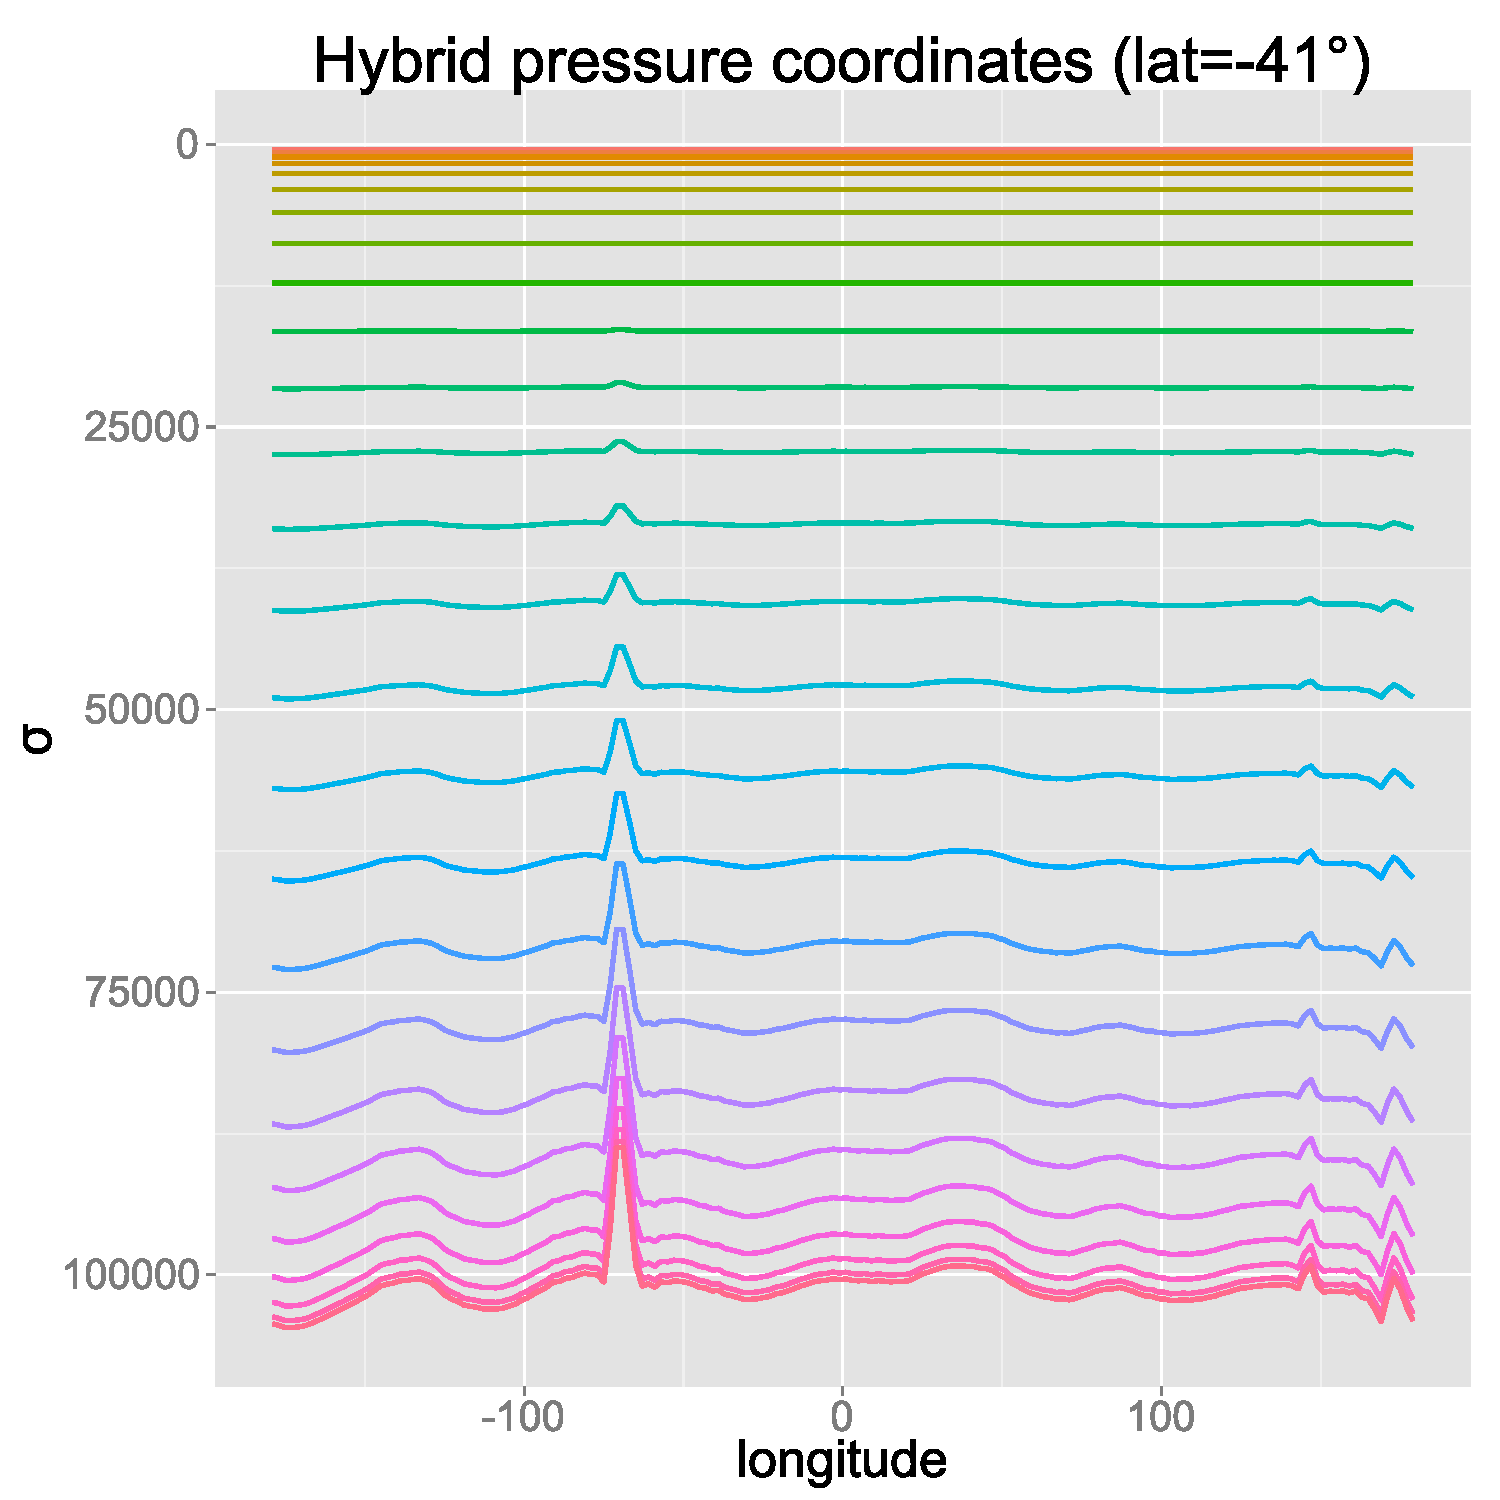
\includegraphics[width=\linewidth]{hybrid_coordinates.pdf}
    \caption{Hybrid coordinates of MOCAGE at latitude=-41\degree as a function of
      longitude. For readability purposes, not all levels are shown here (roughly
    one over two). The largest peak corresponds to the Andes mountains.}
\label{fig:hybrid}
  \end{minipage}
  \hfill
  \begin{minipage}[t]{0.45\linewidth}
    \centering
    \includegraphics[width=\linewidth]{grids_formats.pdf}
    \caption{Workflow for the input data: MOCAGE uses data from the European Center,
    which is then interpolated onto the Pangolin grid.}
\label{fig:grids_formats}
  \end{minipage}
\end{figure}
%

\subsection{Spatial interpolation}
\label{subsec:spatial_interp}
The MOCAGE grid is a three-dimensional regular latitude-longitude grid. We want
to interpolate the ozone concentration, temperature and winds onto the Pangolin
grid, defined in the isentropic surface mentioned above. 

%\subsubsection{Concentration and temperature}
First, we interpolate ozone concentration and temperature as there are both
defined at the center of the Pangolin cells. For each latitude and longitude,
we interpolate vertically the data from the hybrid coordinates to
$\theta=\theta_0$ using cubic splines.  This gives us data on the isentropic
surface but still on regular latitude-longitude grid. To interpolate it
horizontally on the Pangolin grid, we use the SCRIP library
(see~\cite{Jones1997}). Bi-dimensional interpolation on the sphere can be
difficult due to the singular points in spherical coordinates.  SCRIP manages
these difficulties and offers an area-preserving mapping, described in more
details in~\cite{Jones1999}. This is especially interesting for us as the
interpolation preserves the tracer fluxes needed by our finite-volume approach.
SCRIP needs first two netCDF files defining the input and output grids. It then
proceeds to create an intermediate netCDF file for the mapping between the
grids. In the last step, it uses these mappings from the file to interpolate the
data. We used the default parameters of SCRIP, with the exception of the
northern threshold. Above this threshold, a coordinate transformation is used to
perform the intersection search needed by the conservative remapping. Our tests
showed this transformation introduced non physical structures so it was
disabled.

%\subsubsection{Winds}
Our first approach to interpolate winds was to keep using SCRIP\@. However, the
library requires the data to be defined at the centers of the cells. While the
input winds are defined at the center of the latitude-longitude grid, winds in
Pangolin are defined at the interfaces of the cells. To accommodate the
requirements of SCRIP, we defined a \textit{dual grid}
such as the winds in Pangolin is at the center of the cells in this dual
grid. Zonal and meridional winds are set in a fashion similar to the D-grid of
Arakawa (see Fig.~\ref{fig:merid_fluxes}) so a dual grid has to be defined for both
zonal and meridional winds. Zonal winds adds a supplementary difficulty as there
must be periodic, a feature not managed by SCRIP\@. To bypass this issue, zonal
interpolation was done in two times. First, the latitude-longitude grid was
shifted such as the westmost zonal values were interpolated correctly. The
input grid was shifted back to its initial position to interpolate the other
values. Finally, periodicity was enforced manually for the eastmost zonal
values. 

Unfortunately, this approach proved to generate interpolation artefacts in the
simulation results when resolution was quite small ($0.3\degre$ at the Equator).
As winds do not need the area-preserving mapping from SCRIP and as the other
interpolation schemes provided by SCRIP cannot accommodate a non-regular
structure, we chose another, simpler interpolation technique. The idea is to use
successive 1D interpolations with cubic splines. The algorithm is detailed
in~\ref{algo:winds_interp}. We first construct an initial array of interpolated
value at each latitudes, and then interpolate the final values from it.

\begin{algorithm}
  \caption{Winds interpolation}
\label{algo:io_seq}
  \begin{algorithmic}
    \Require 2D winds array $u$ on lat-lon grid
    \Ensure 2D winds array $U$ on Pangolin grid
    \State Skip all latitude lines up to $first\_line$
    \ForAll{$\phi_i$ in Pangolin}
      \ForAll{$\lambda'_j$ in lat-lon}
      \State $u'(\lambda'_j) = $ cubic interpolation on $u$ for all latitudes in
      lat-lon
      \EndFor
      \ForAll{$\lambda_j$ in Pangolin}
        \State $U(\phi_i, \lambda_j) = $ cubic interpolation on $u'$ for all
        longitudes in lat-lon
      \EndFor
    \EndFor
  \end{algorithmic}
\label{algo:winds_interp}
\end{algorithm}

\subsubsection{Programming details}
From a software point of view, we created a small external preprocessing tool which
takes a 3D latitude-longitude grid as input in the netCDF format and interpolate
it to a 2D isentropic Pangolin grid in HDF5. The workflow is illustrated on
Fig.~\ref{fig:grids_formats}. For horizontal interpolation, the
subroutines from SCRIP are called directly instead of running the executable for
each timestep and for each data. Also, the mapping between the latitude-longitude and
the Pangolin grid are only created once.

\subsection{Description of MOCAGE}
\label{subsec:mocage}
MOCAGE is the three-dimensional CTM developed and used by M\'et\'eo-France, the
French weather forecast agency.  It is used in data assimilation experiments
(\cite{Cathala2003}), where the output of models is combined statistically with
observations, taking into account the incertitudes.  It can also be used for
chemical weather forecasting, where meteorological data is given to the CTM,
which in turns forecasts the evolution of the chemical composition of the
atmosphere. One application of this is air quality forecasts.

MOCAGE uses a semi-Lagrangian scheme based on~\cite{Williamson1989} for
advection. It includes the stratosphere and the troposphere and various
chemistry schemes can be used, from simplified linearized schemes up to detailed
schemes including gas-phase and heterogeneous stratospheric and tropospheric
chemistry (\cite{Lefevre1994}). The input winds and temperature come either from
ARPEGE, the operational global model of M\'et\'eo-France, or from the
\gls{ECMWF} analyses or forecasts.

In our study MOCAGE and Pangolin are forced using the \gls{ECMWF} operational
analyses. MOCAGE uses is a bi-dimensional latitude-longitude grid with 60
vertical levels in hybrid coordinates. The time-step for advection is set to 1h,
while the chemistry time-step is set to 15min. A complete description of the
MOCAGE model is given by~\cite{Josse2004}.

\subsection{Linear chemistry}
The global evolution of the tracers is a CTM is the sum of many physical
processes, where the most important in the stratosphere are advection and chemistry
operators. This can be implemented by integrating in time both advection and
chemistry directly. The different natures of the associated operators make that
strategy especially difficult.  Instead, a most common method is adopted where
the temporal integration is carried out successively for each process over a
series of time-step. The advection operator gives an intermediate
tracer evaluation, which is then fed to the chemistry operator, resulting in the final
tracer value at the end of the time-step. As this strategy introduces a
splitting error, a scheme with alternate directions (in a way similar to the
strategy presenting for the advection) can be used in practice. 

Here, we focus on the chemistry scheme. Interactions between the different
chemical species lead to the resolution of a set of coupled \glspl{ODE}.
Unfortunately, the chemical species in the atmosphere have very different
lifespans, ranging from milliseconds to several weeks. The set of equations is
then said to be \textit{stiff} so the usual explicit methods do not work: the
global time-step of the system will be set as the smallest time-step of the
system, which is too constraining. Several methods can be used to bypass this
issue. Quasi-Steady States Approximations is a method presented
by~\cite{Hesstvedt1978}, which has the advantage of being positive and allowing
larger time-step. Unfortunately, it does not guarantee mass preservation.
Another approach by~\cite{Verwer1994} is called \enquote{two-steps backwards}. For a
comparison between the different methods, the reader can refer
to~\cite{Sandu1996}. 

To simplify the problem and concentrate on comparison between MOCAGE and
Pangolin, we have chosen instead to use a linear scheme for ozone. Such a
scheme was developed by~\cite{Cariolle2007} and has proved to be well
adapted for ozone simulation in the stratosphere. With this scheme, the ozone
continuity equation writes:
\begin{equation*}
  \frac{\partial r_{O_3}}{dt} = P-L,
\end{equation*}
where $r_{O_3}$ is the ozone mixing ratio, $P$ and $L$ are the production and
loss rate respectively. The equation is expanded using a Taylor serie to:
\begin{align}
  \frac{\partial r_{O_3}}{dt} &= A_1 +A_2(r_{O_3}-A_3)+A_4(T-A_5) 
  +A_6 (\sigma -A_7)+A_8 r_{O_3},
\label{eqn:chem_taylor}
\end{align}
where the $A_i$ are monthly-averaged coefficients (the overlay denotes the
average):\\
\begin{tabular}{ll}
$A_1=\overline{P-L}$ & $A_5=\overline{T}$: temperature \\
$A_2=\frac{\partial \overline{P-L}}{\partial r_{O_3}}$ & $A_6=\frac{\partial \overline{P-L}}{\partial \sigma}$\\
$A_3= r_{O_3}$ & $A_7=\sigma$: ozone column \\
$A_4=\frac{\partial \overline{P-L}}{\partial T}$ & $A_8$: heterogeneous chemistry term\\
\end{tabular}\\
More precisely, the coefficient are given by MOBIDIC, a bi-dimensional
photochemical model developed by~\cite{Cariolle1985}. The model was run for the
year 2000 and its coefficients are used as if for the year of our simulation
(2008). 
For our study, only the first five terms ($A_1$ to $A_5$) are taken into account
in the Pangolin simulation. This means that the ozone concentration will be
sensitive to temperature, but not to the ozone column above the chosen potential
temperature surface. Equally, the potential impact of heterogeneous chemistry is
not taken into account. 

A semi-implicit scheme is then used to discretize Eq.~\eqref{eqn:chem_taylor} as
it allows for a larger time-step and preserve the positivity of the ozone
concentration. The equation becomes:
\begin{equation*}
  \frac{r_{O_3}^{n+1} - r_{O_3}^n}{\Delta t} = A_1 +A_2(r_{O_3}-A_3)+A_4(T-A_5), 
\label{eqn:chem_taylor}
\end{equation*}
leading to
\begin{equation*}
  r_{O_3}^{n+1} = \frac{r_{O_3}^n + \big(A_1 -A_2 A_3 + A_4 (T^n-A_5)\big)\Delta t}
  {1-A_2\Delta t},
\end{equation*}
where $T^n$ is the temperature at time-step $n$ and $\Delta t$ the corresponding
time-step.

\section{Results}
\label{sec:results_final}
\defcitealias{NCL}{NCL reference manual}
\defcitealias{Kennison2014}{NCL documentation}
We present here the results of a run of Pangolin over one month, both with and
without chemistry. The simulation is run from September, 1\textsuperscript{st}
2008 to October 1\textsuperscript{st} 2008. MOCAGE uses a 3D regular
latitude-longitude grid, with 60 vertical levels and a horizontal resolution of
$2\degre\times2\degre$. Several resolutions have been tested with Pangolin. The
coarser grid has a resolution of $2.9\degre \times1.96\degre$ at the equator,
close to the one of MOCAGE\@. The same time-step of 30 min is used for both the
chemistry and advection. The finer grids tested have resolutions of $1.5\degre
\times1.0\degre$ and $0.5\degre \times0.33\degre$.

To ensure the horizontal interpolation of Section~\ref{subsec:spatial_interp}
are accurate, we compare the initial ozone concentrations interpolated on the
Pangolin grid to its equivalent on the MOCAGE grid. To make the comparison
relevant, the MOCAGE data is interpolated on the same isentropic coordinate as
Pangolin. Results are shown on Fig.~\ref{fig:31lat_0}. It should be noted that
the plot is done using the NCL software (see the~\citetalias{NCL}), which adds
another interpolation when creating a contour plot on an irregular grid. The
algorithm consists in creating a triangulation of the initial grid and creates
the contour from the triangulated mesh (see~\citetalias{Kennison2014}). From
the figure, it can be seen that the horizontal interpolation provides close
results with the initial data. With the exception of the smallest structures,
the various shapes of the ozone field are well-preserved.  As expected, some
structures are lost near the poles due to the smaller number of cells of
Pangolin.
\begin{figure}
  \subbottom{%
    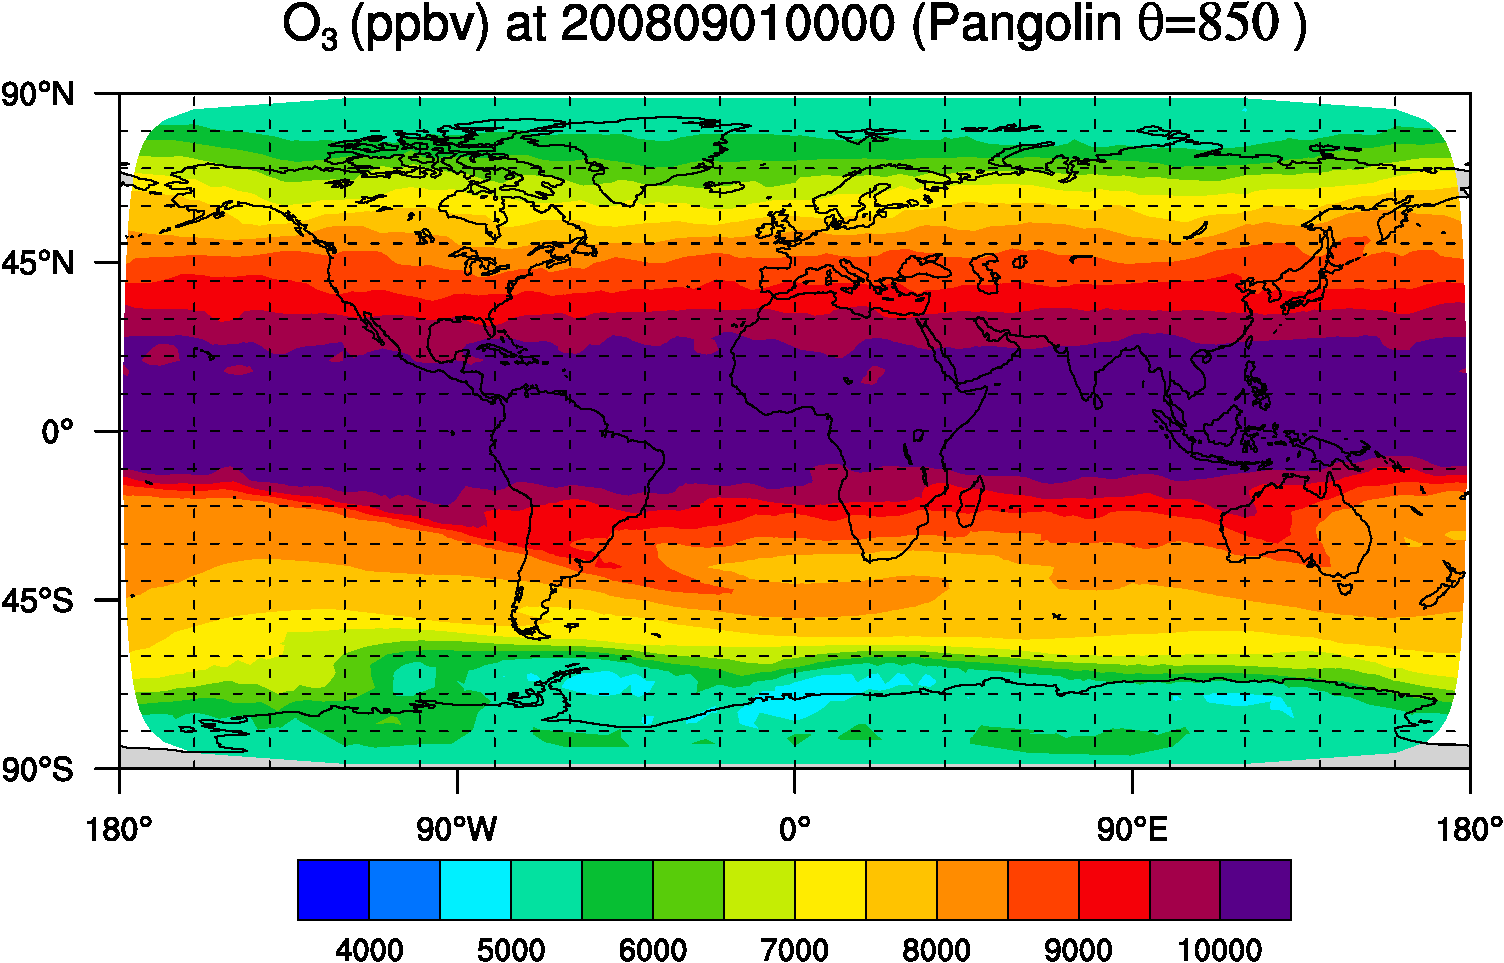
\includegraphics[width=0.8\linewidth]{pangolin_31lat_2008090100.pdf}
  }
  \hfill
  \subbottom{%
    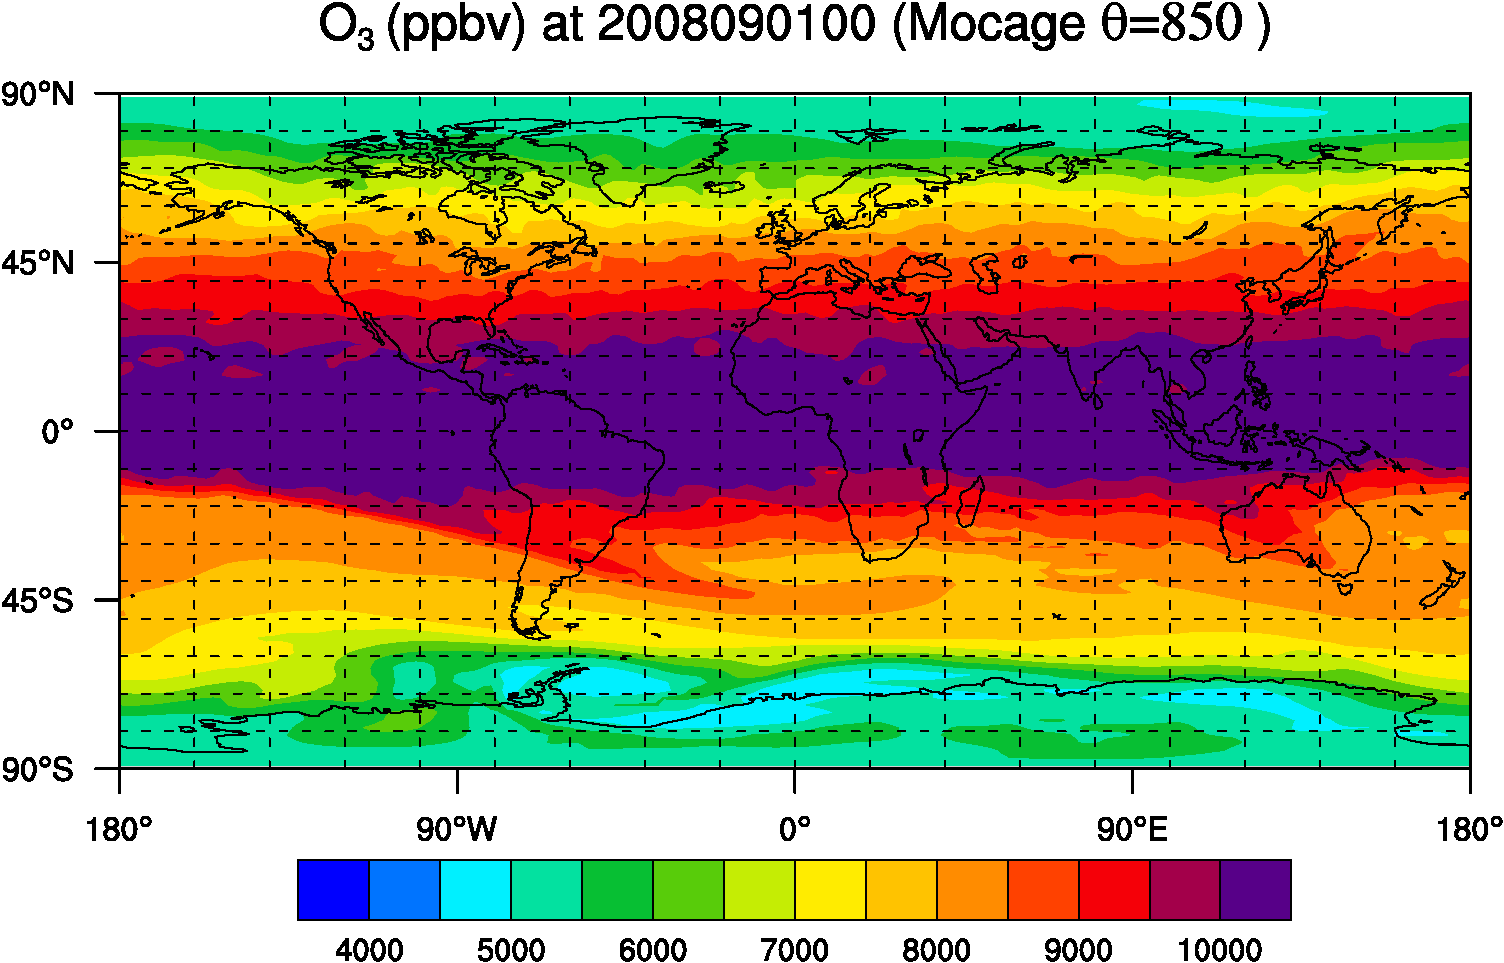
\includegraphics[width=0.8\linewidth]{mocage_2008090100.pdf}
  }
  \caption{Comparison of the initial distributions for Pangolin and MOCAGE\@. Both
  are interpolated on the isentropic surface $\theta=850$K.  Ozone
  concentrations are given in particles per  billion per volume (ppbv).}
\label{fig:31lat_0}
\end{figure}

We first examine the results of resolution on Pangolin for advection only.
Here, and in the following results, the winds are corrected and the
shape-preserving limiter is enabled. Results after one month are shown
on~Fig.\ref{fig:advec_T} for the various resolutions.  It can be seen that the
increase in resolution allows smaller structures to appear, such as the vortex
in the South Pacific Ocean, and in the South Pole region around the polar
vortex. To ensure these structures had a physical reality and were not the
byproduct of either interpolation or the advection scheme, we thoroughly checked
the output of the simulation every three hours. The structures formed of
filaments result from elongation of the tracer in region of strong wind
shear. This occurs in particular in the transition regions between the
equatorial easterlies and polar westerlies. This situation is what can be
expected from quasi-2D turbulence where tracers present filamentary structures
in presence of large scale vortices. 

The same simulations with the chemistry enabled are shown on
Fig.~\ref{fig:chem_T}. The plots show that chemistry plays an important role in
the redistribution of the ozone concentration. Despite that all the structures
induced by advection are still visible, their amplitudes are `smoothed out' by
chemical production or destruction with a tendency to relax the concentrations
towards the climatological values of the linearized scheme.

\begin{figure}
  \centering
  \subbottom[$2.90\times1.97\degre$]{%
    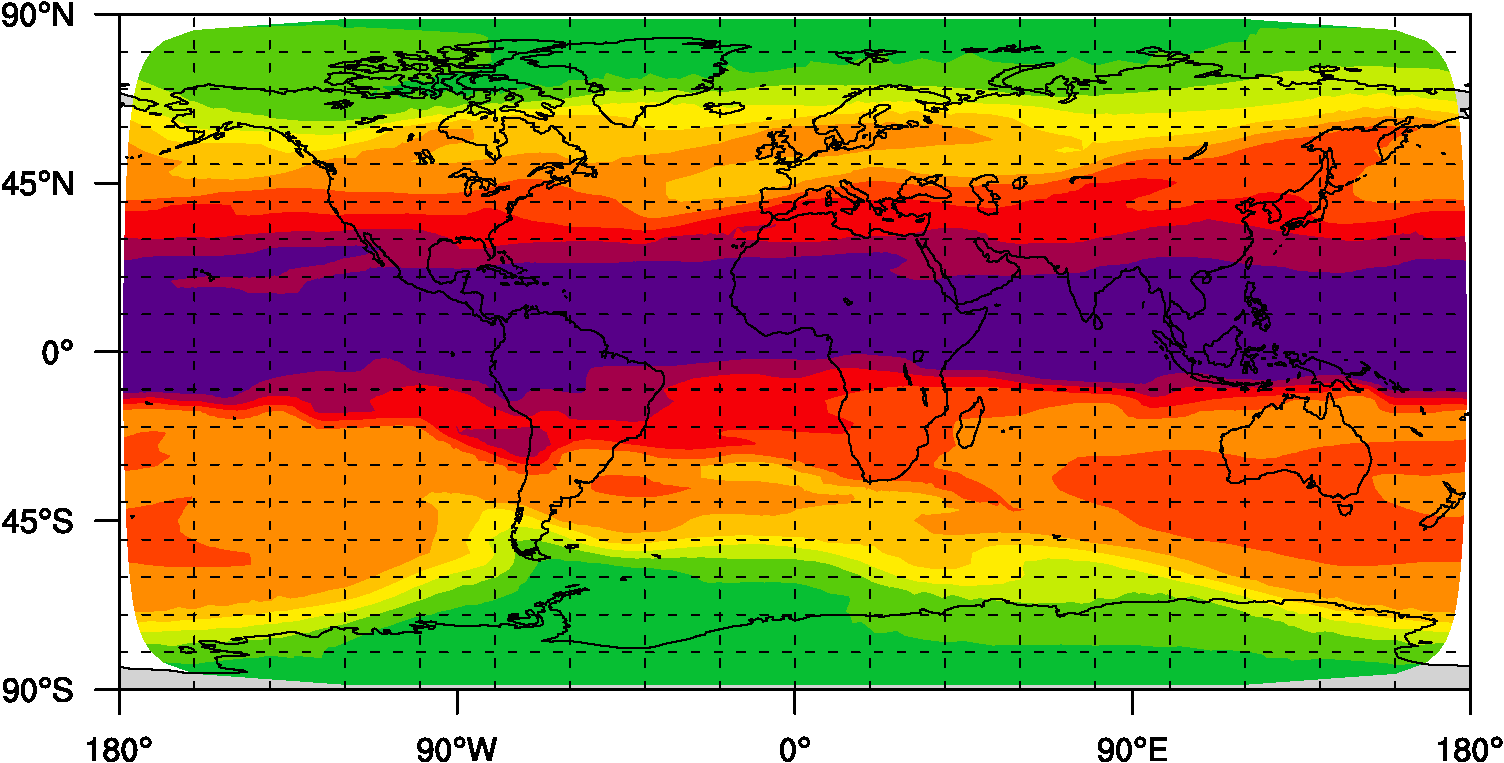
\includegraphics[width=0.8\linewidth]{pangolin_31lat_advec_2008100100_cut.pdf}
  }
  \hfill
  \subbottom[$1.5\times1.00\degre$]{%
    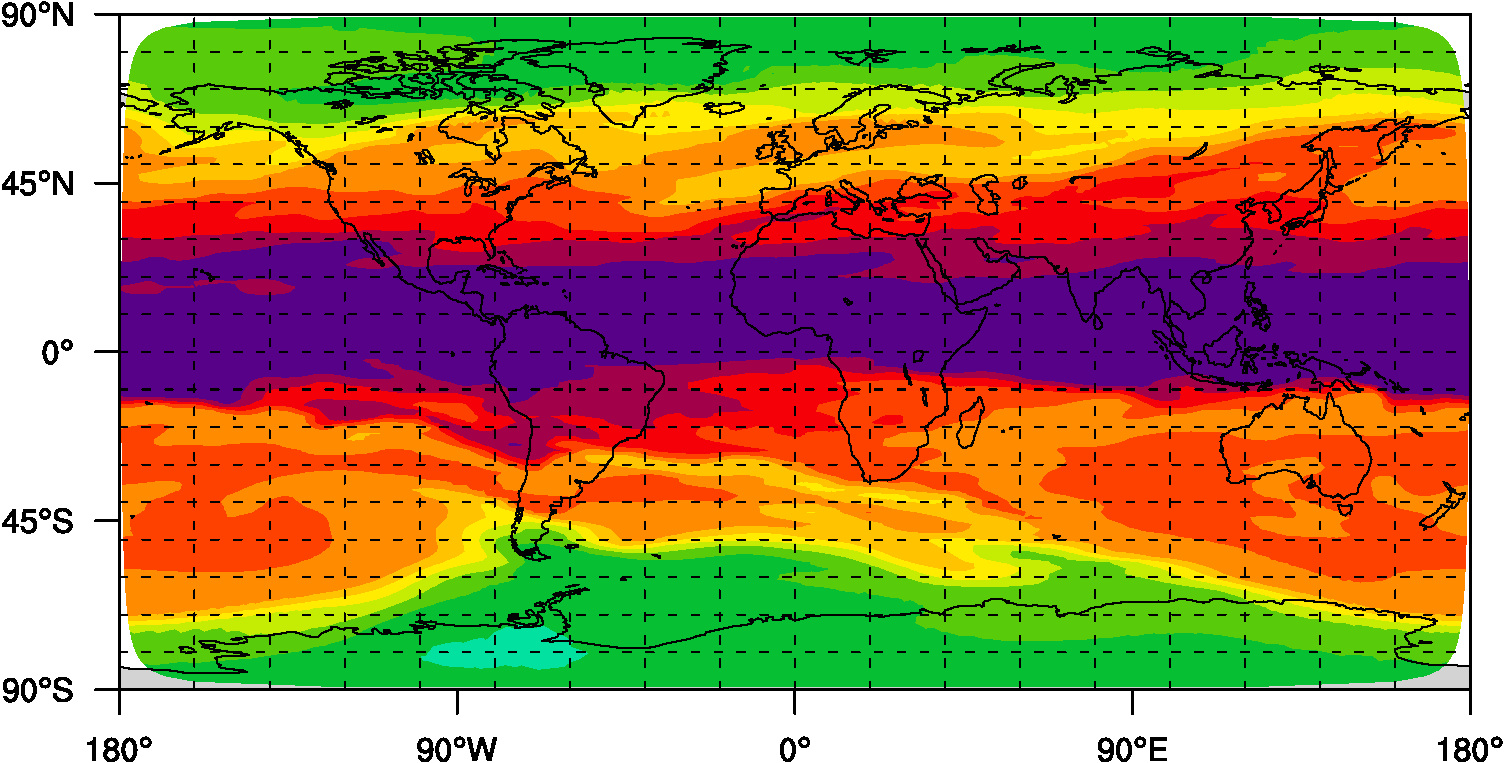
\includegraphics[width=0.8\linewidth]{pangolin_60lat_advec_2008100100_cut.pdf}
  }
  \hfill
  \subbottom[$0.5\times0.33\degre$]{%
    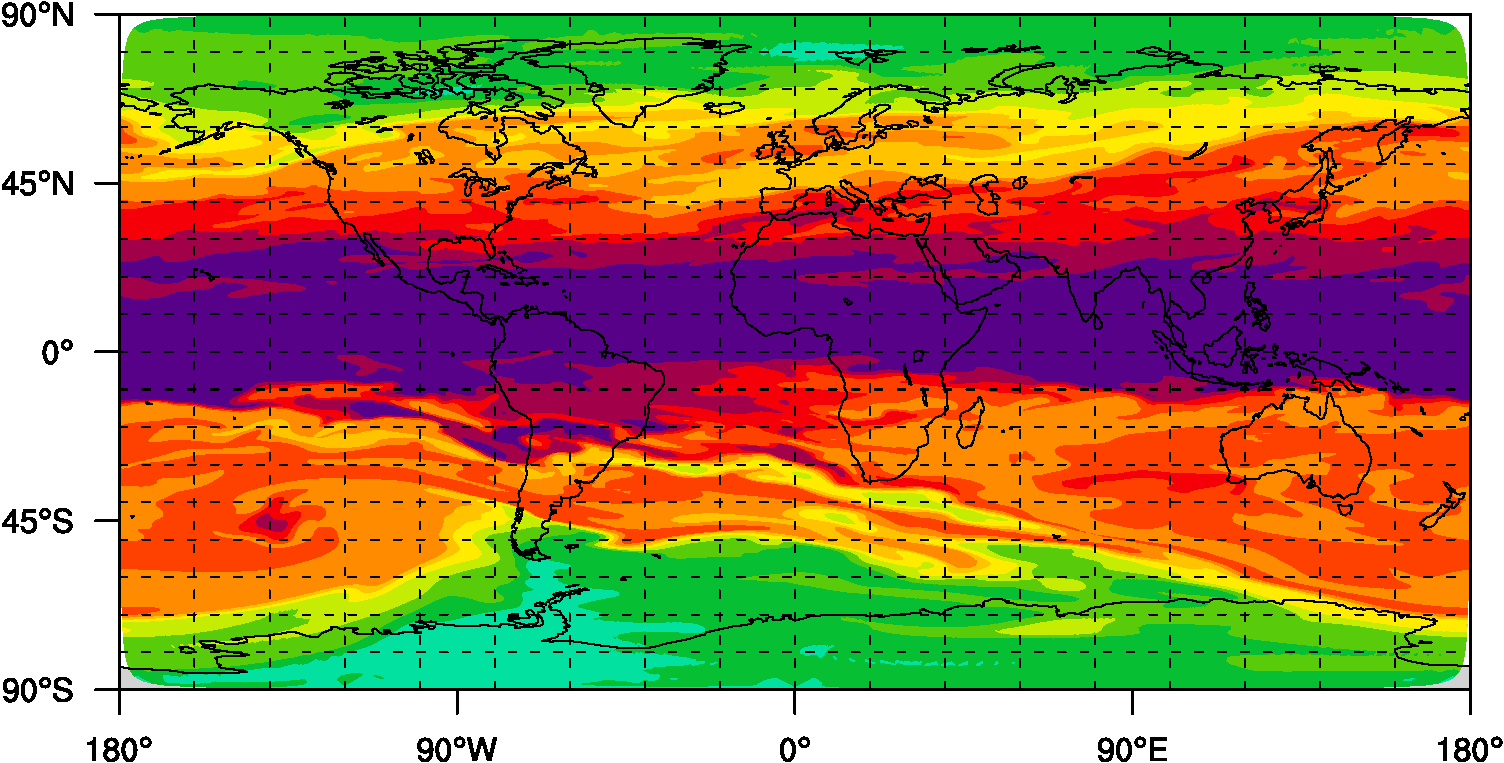
\includegraphics[width=0.8\linewidth]{pangolin_180lat_advec_2008100100_cut.pdf}
  }
  \caption{Impact of resolution on ozone distribution after a month with
  Pangolin. Only advection is enabled and the results are shown on the isentropic
  surface $\theta=850$K. The legend is the same as on Fig.~\ref{fig:31lat_0}.}
\label{fig:advec_T}
\end{figure}

\begin{figure}
  \centering
  \subbottom[$2.90\times1.97\degre$]{%
    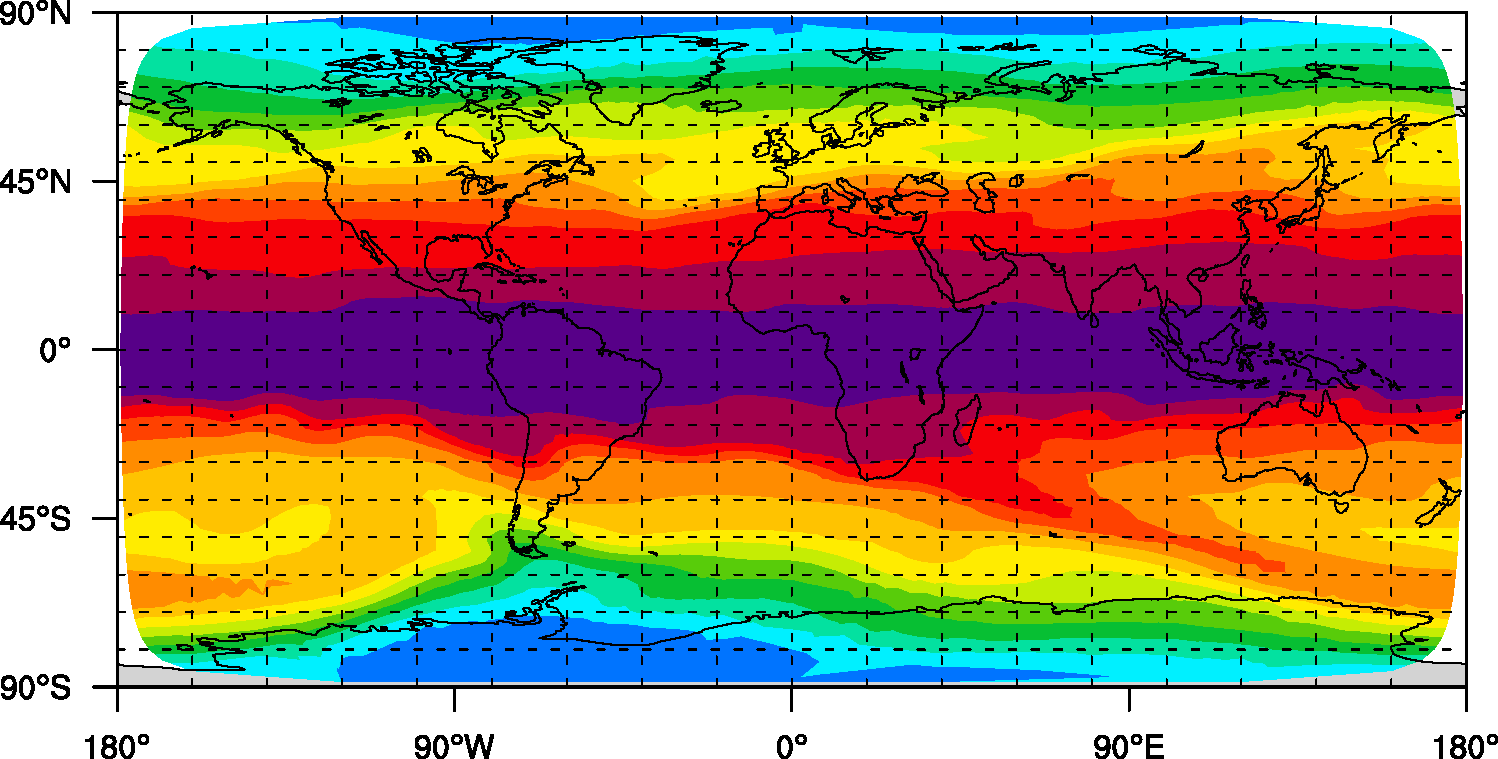
\includegraphics[width=0.8\linewidth]{pangolin_31lat_chem_2008100100_cut.pdf}
\label{fig:chem_31lat_T}
  }
  \hfill
  \subbottom[$1.5\times1.00\degre$]{%
    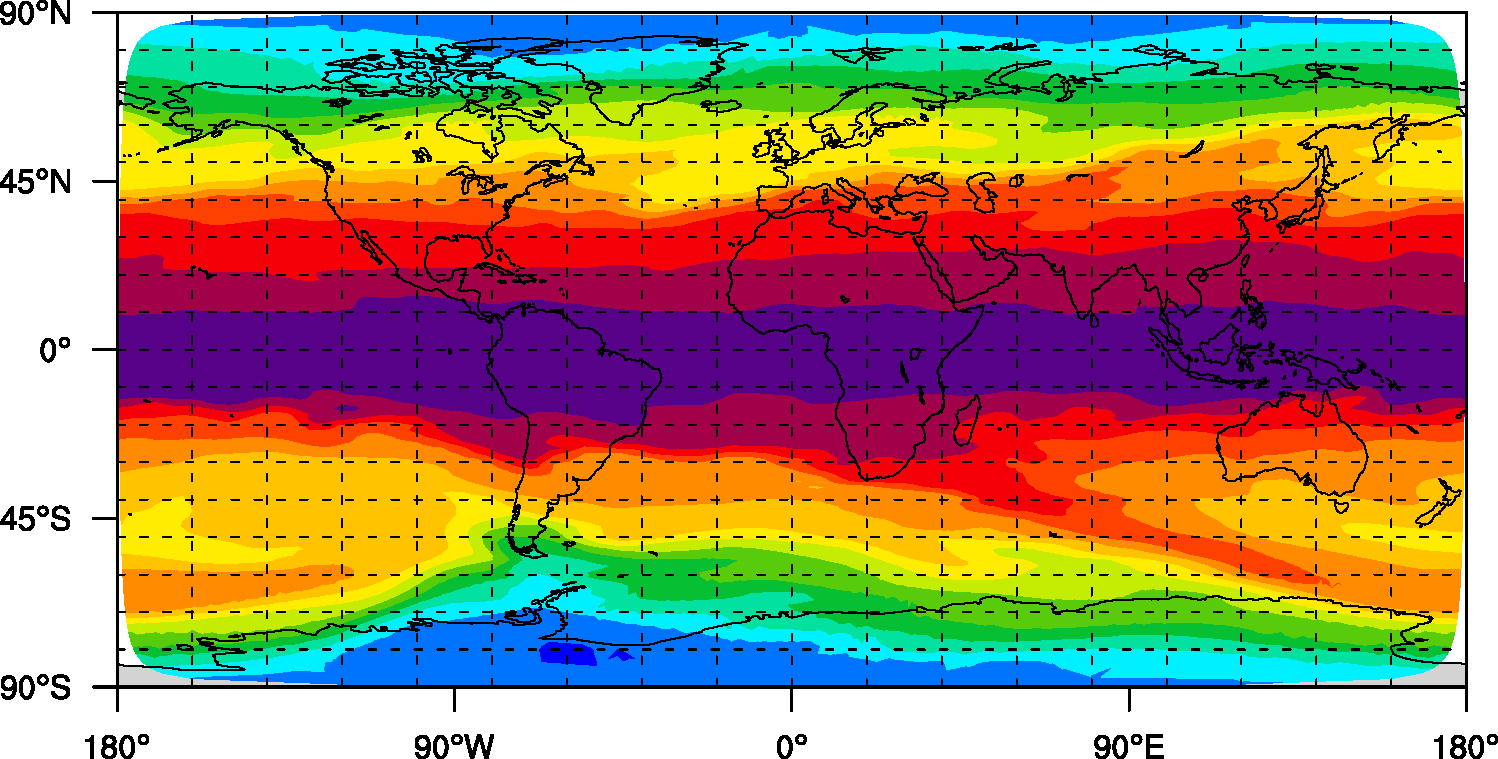
\includegraphics[width=0.8\linewidth]{pangolin_60lat_chem_2008100100_cut.pdf}
\label{fig:chem_60lat_T}
  }
  \hfill
  \subbottom[$0.5\times0.33\degre$]{%
    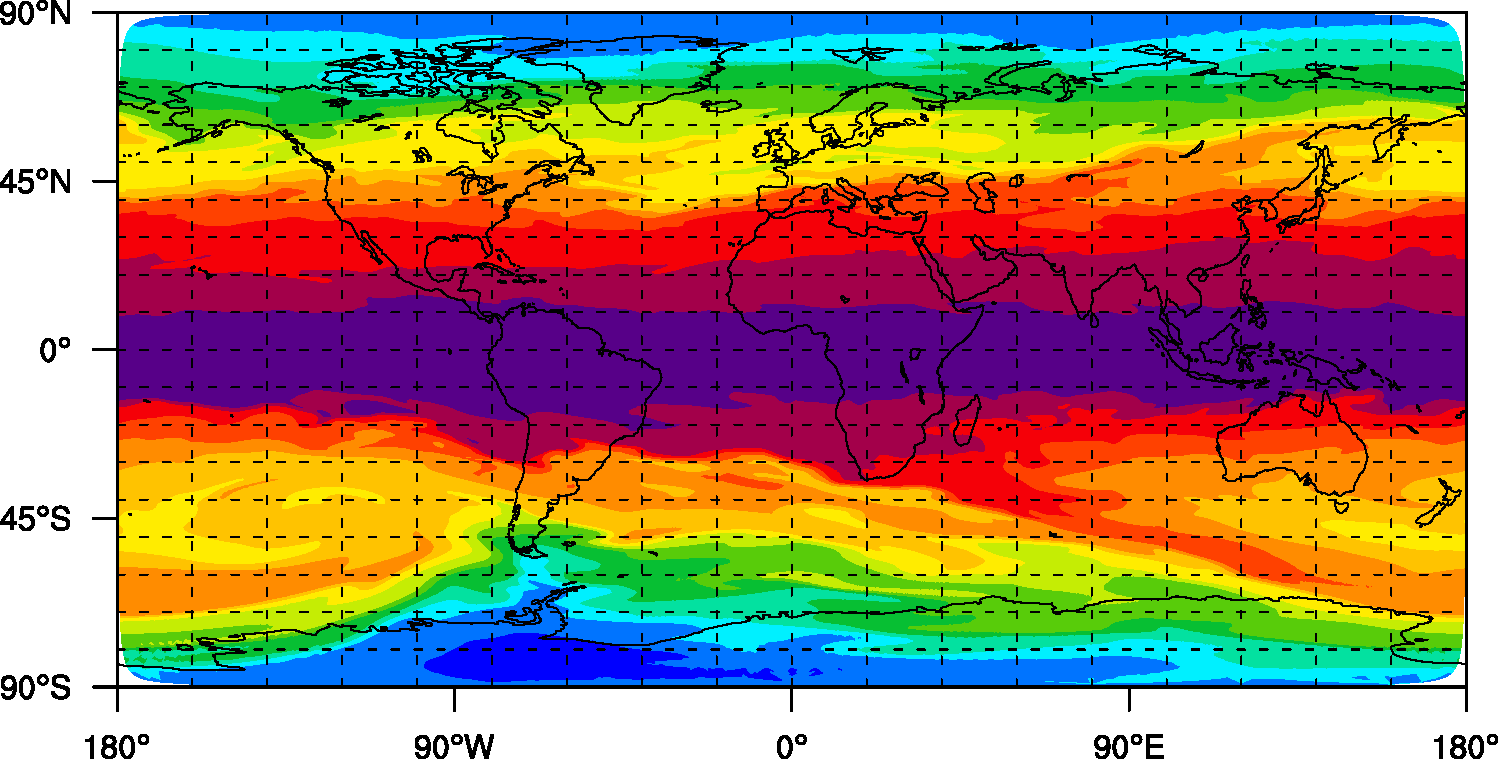
\includegraphics[width=0.8\linewidth]{pangolin_180lat_chem_2008100100_cut.pdf}
\label{fig:chem_180lat_T}
  }
    \caption{Impact of increasing resolution on the ozone distribution after a
      month with Pangolin. Both advection and the linear ozone scheme are
      enabled and the results are shown on the isentropic surface
      $\theta=850$K. The legend is the same as on Fig.~\ref{fig:31lat_0}.}
\label{fig:chem_T}
\end{figure}

The output of MOCAGE at the end of the simulation is shown on
Fig.~\ref{fig:mocage_T}. With a resolution similar to MOCAGE, Pangolin is able
to match the larger structures after a month (Fig.~\ref{fig:chem_31lat_T}). With
twice the resolution (Fig.~\ref{fig:chem_60lat_T}), medium-scale structure are
correctly modelled by Pangolin, such as the vortex in the South Pacific Ocean
mentioned before or the long filament south of Australia. With a resolution six
times finer (Fig.~\ref{fig:chem_180lat_T}), some small-scale structures are
reconstructed by Pangolin, like in western Russia, above Japan or north of
Chile. However, much of the smaller structures do not appear on the MOCAGE
simulation as the resolution is too coarse for such levels of details. Also, the
difference in the North pole can be explained
by the difference in the chemistry scheme: MOCAGE uses actually all the terms
from Eq.~\eqref{eqn:chem_taylor}, while Pangolin uses only the first five. Also,
the radiative balance is not perfect over the poles due to the lack of solar
heating that does not counterbalance the infrared cooling, so the motions are
not completely adiabatic. This means that vertical advection can play a larger
role and the comparison of the model outputs on isentropic surfaces can only be
qualitative. Nevertheless, we can conclude from these tests that Pangolin gives
quality simulations for 2D advection and can be an alternative to MOCAGE if used
with sufficient resolution.  This result validates our strategy since high
resolutions can be easily implemented within Pangolin due to its good
performances running on parallel computers. 

\begin{figure}
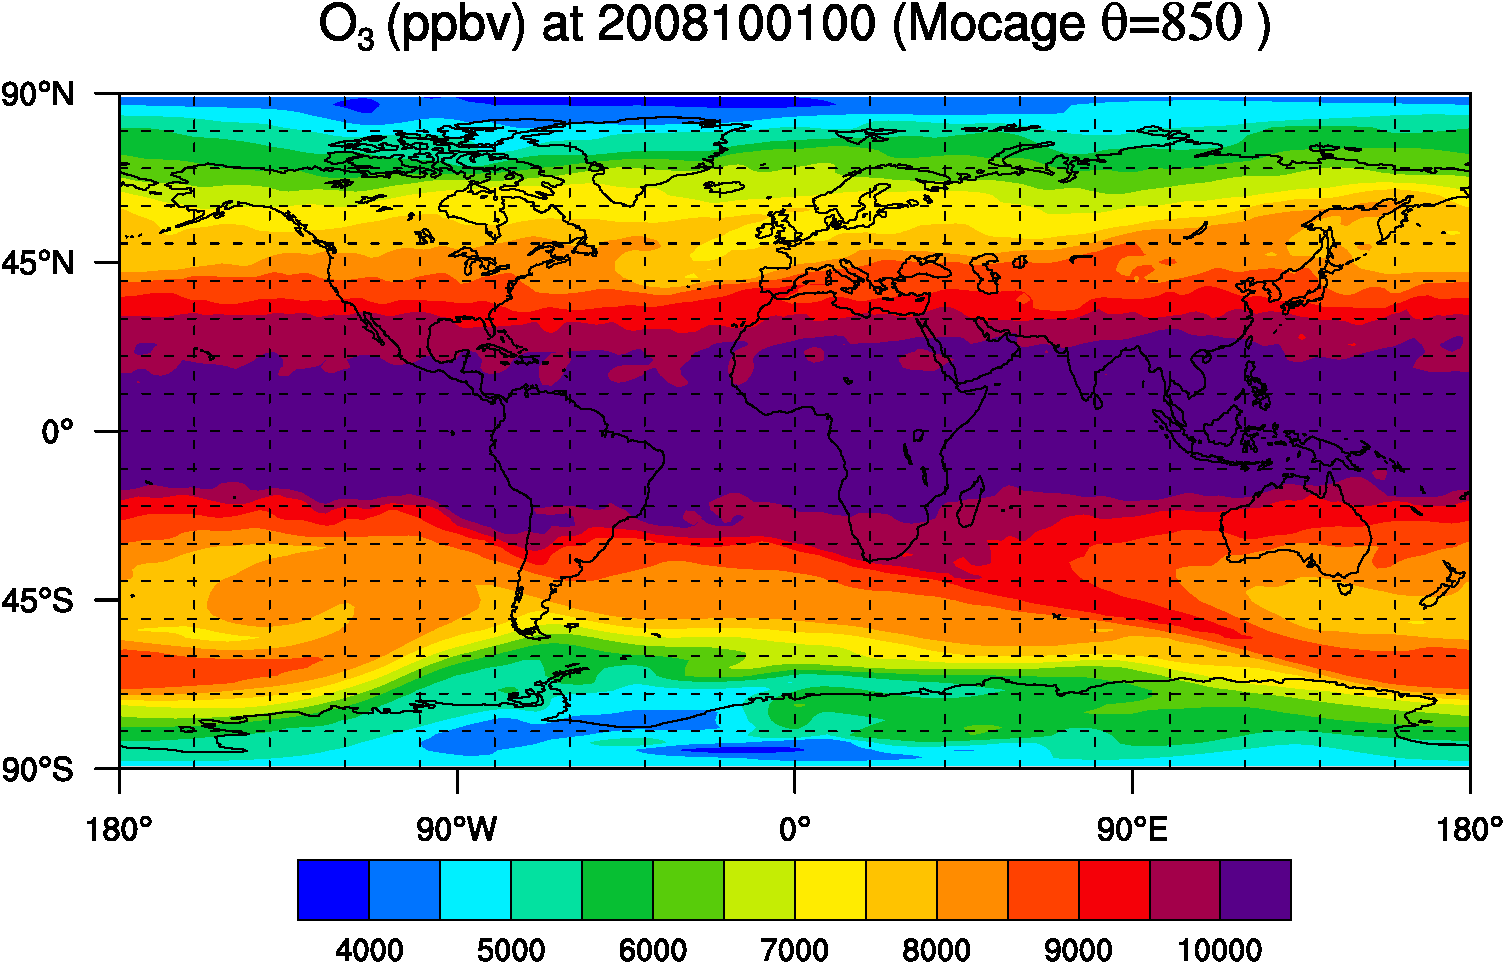
\includegraphics[width=\linewidth]{mocage_2008100100.pdf}
\caption{Ozone distribution after a month with MOCAGE with a resolution of
  $2\degre\times2\degre$. The output is interpolated on isentropic coordinates
$\theta=850$K.}
\label{fig:mocage_T}
\end{figure}

